The inflation gas is key to providing the structural stiffness for the inflatable: it is required to bring all members into tension to prevent skin wrinkling under compressive loading. To this end, the aeroshell will require an inflation system that is reliable, lightweight and fitting within mass and volume constraints. This subsection details the selection of an inflation gas and design of the inflation system upon which aeroshell deceleration capability hinges.

\paragraph{Gas generator selection}
Inflation systems can be categorized as tanked-gas systems, phase-change systems and chemical gas-generation systems \cite{Jenkins2001}. These systems have each been considered for their respective advantages, yielding a tanked nitrogen inflation system as outcome. 

%\paragraph{Phase-change system}
Phase-change systems have the potential to provide significant mass reductions. The most promising option is a liquid hydrogen inflation system, while other phase-change systems involve subliming powders, although these are incapable of achieving high pressures \cite{Freeland1998}.  On the basis of system mass fractions investigated by Brown et al. \cite{Brown2009} and the mass estimation tool detailed in section \ref{subsec:structool}, a structural mass reduction of nearly 20 [$kg$] is deemed feasible with a cryogenic liquid hydrogen inflation system following from the mass estimation tool formulated in section \ref{subsec:structool}. 


This mass reduction comes at the expense of reliability, however. These systems involve a phase-change process, inherently unpredictable and thereby accompanied with reduced inflation system reliability \cite{Jenkins2001}. In addition, cryogenic storage requires profound thermal control to keep it below its required temperature. While this poses a challenge for orbiting satellites, it is even more so an issue in the heated re-entry environment of the inflatable aeroshell. Reliability is further lessened by the absence of successful efforts in the past to accommodate a phase-change inflation system in spaceflight, let alone a high-pressure application like the aeroshell at hand. As reliability is key for transporting human payload, phase-change systems are deemed ill-suited. Moreover, a liquid hydrogen inflation system poses issues for safety when operating in the Earth atmosphere, in which flammability risk is present by the dual presence of hydrogen and oxygen in a heated environment. Re-entry on Earth should be considered for possible return missions of the inflatable aeroshell.


%\paragraph{Chemical gas-generation system
Chemical gas-generation systems similarly feature a higher level of complexity and thereby lower level of reliability than tanked-gas systems \cite{Jenkins2001}. Moreover, while mass reductions are deemed feasible, these involve the use of hydrazine \cite{Jenkins2001, Freeland1998}. Hydrazine poses issues with respect to cost and handling, but most importantly with respect to sustainability. As the decelerator will make contact with a hard surface, leakage of hydrazine into the Martian atmosphere and pollution of the landing site by its toxic nature poses a risk. This risk would violate \gls{cospar} regulations and moreover limit the sustainable dimension of the mission.

Tanked-gas systems are the preferred choice, featuring a significantly higher level of reliability and past application. Most notably, these have seen application in the \gls{irve} missions in the form of a nitrogen blow-down system \cite{Smith2010}. Blow-down systems offer controllable gas flow at low development and hardware cost \cite{Freeland1998}. Moreover, these are excellently suited for high-pressure applications in inflatable structures \cite{Jenkins2001}.

Using helium rather than nitrogen would be infeasible. Due to the small size of helium atoms, permeability of the tank and inflatable becomes an issue and pressure leakage a more pronounced phenomenon. Moreover, helium application in spacecraft applications has remained uninvestigated in literature and thereby poses significantly higher development risk.


\paragraph{Gas generator design and sizing}
A nitrogen tank is used for storage and supply of nitrogen gas. The minimum inflation pressure in the toroids is based on the premise that it should counteract the aerodynamic force exerted to bring flexible material into tension, formulated in Equation \ref{eq:Pmin}. The volume that is inflated may be approximated as the sum of the volumes of separate toroids summated over the entire sphere cone.

From the structural analysis it followed that a pressure of 3.9 [$kPa$] over a total volume of 68 [$m^{3}$] is required in the inflatable bladders. This minimum inflation pressure is smaller than that required in \gls{irve}-3 \cite{Jurewicz2011}, hence it induces smaller loads, which make up most of the flexible wall loading and the structural lay-up can consequently be thinner than in the case of \gls{irve}-3. The inflation pressure brings all members into tension, as illustrated by Figures \ref{fig:strucl} and \ref{fig:strucs}.

To account for pressure losses following from a drop in temperature, as observed in the \gls{irve}-II mission \cite{Dillman2012}, a heater is used to heat the tank after partial usage of the inflation gas. The total mass of the inflation gas can be estimated on the basis of the required operating pressure. From a functional perspective the minimum required inflation pressure should be reached at all phases of the deceleration. Thermal loading of the aeroshell will increase the temperature of the inflation gas and cause a proportional increase in pressure. Pressure increases above the minimum inflation pressure are beneficial as this will increase the stiffness of the aeroshell. This works up to some point as structural loading has to be taken into account as well. If the pressure increases to much venting may be performed to reduce the pressure, which will be further discussed in the subsequent paragraph. Pressure decreases below the minimum required pressure are however dangerous as the stiffness of the aeroshell will be lost.

For this reason a minimum operational temperature is considered. Figure \ref{fig:tanktemp} shows the temperature range in Kelvin for a cylindrical body emitted by the sun from the side around Mars. The temperature is based on heat flow equilibrium, not considering any of the atmospheric entry effects \cite{Wertz2011}. A range of absorptivity over emissivity values is considered. This value is dependent on the outer coating of the spacecraft and is an large extend left free to be chosen. Nevertheless a conservative value of 0.5 is chosen which yields a temperature of 202 [$K$]. Lower temperature increases are not envisioned for a threefold of reasons:

\begin{itemize}
\item The Martian atmospheric temperature ranges between 100 and 200 [$K$], but conduction is low and only for the short period within the Martian atmosphere
\item Solar radiation will still heat the re-entry vehicle
\item Thermal loading will cause an increase in temperature even after the heat shield of the inflatable.
\end{itemize}

\begin{figure}[h]
		\centering
		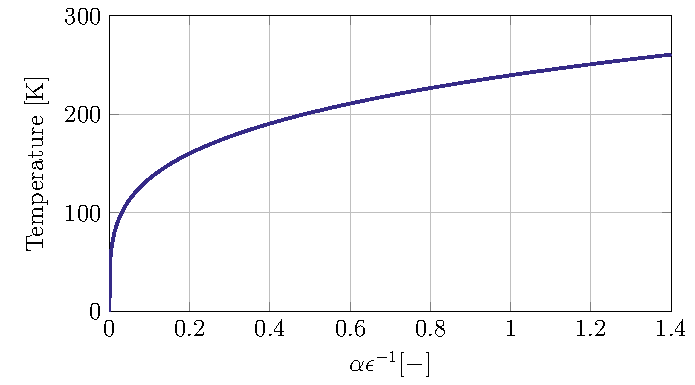
\includegraphics[width=0.7\textwidth]{./Figure/Structure/Temp.pdf}
		\caption{Temperature range for a cylinder at Mars as function of the absorptivity over emissivity}
		\label{fig:tanktemp}
\end{figure}

Using a temperature of 202 $[K]$ inside the inflatable yields a total gas mass of 90 $[kg]$ that is to be held within the pressure tank, given a molar mass of 22 $[g\cdot mole^{-1}]$ for nitrogen gas \cite{Samareh2011}. An additional contingency of $20\%$ is included. This contingency accounts for leakage, which requires additional gas to make up for the lost volume, so called make up gas \cite{Jenkins2001}.

The ratio of tank and inflatable volume is obtained via the ideal gas law as:

\begin{equation}
\frac{\gls{sym:vol}_{tank}}{\gls{sym:vol}_{inflatable}} = \frac{P_{infl}T_{tank}}{P_{tank}T_{infl}}
\label{eq:volratio}
\end{equation}

Initial estimates for the tank pressure and temperature are 27.6 $[MPa]$ and 323 $[K]$ \cite[p.545]{Wertz2011}. Based on the required pressure and a temperature of 202 $[K]$ in the inflatable, by use of the ideal gas law, a total pressure tank volume of 0.27 $[m^{3}]$ follows. Corresponding to this tank volume is a required tank mass, dependent on the material used. Composite overwrapped pressure vessels offer significant weight advantages with respect to metallic tanks and therefore such a pressure vessel is selected. Tank mass is estimated from empirical relations established by Zakrwski \cite[p.546]{Wertz2011} to be 61 $[kg]$ for the selected tank pressure and volume via Equation \ref{eq:tmass}.
\begin{equation}
m_{tank} = 0.7266 \cdot (P_{tank} \cdot \gls{sym:vol}_{tank})^{2} + 2.5119 \cdot (P_{tank} \cdot \gls{sym:vol}_{tank}) + 2.9826
\label{eq:tmass}
\end{equation}

\paragraph{Inflation system integration}

Figure \ref{fig:infsys} shows a schematic representation of the inflation system. The inflation gas is stored in a nitrogen tank. Pressure and temperature sensors are included to monitor the storage conditions. A separate valve is included for filling purposes of the tank, and a release valve is included for emptying the tank outside normal mission operations. A electromechanical valve releases the pressure. A electromechanical valve is used since it allows for multiple uses as opposed to one-time use pyrotechnical valves, used in early \gls{irve} installments \cite{Hughes2005}. From the high pressure within the storage tank the controlled the pressure is reduced and more precisely controlled by a set of two pressure regulators (including internal release valves). One of the pressure regulators is located in the high-pressure part of the inflation system in the centerbody, the other in the low-pressure part. Duality of pressure regulators accounts for flow adjustment while also taking into account feed losses. A set of check valves, allowing flow only in one direction, connects to the toroid. Purpose thereof is to prevent flow from exiting the bladder volumes. 

The toroids are grouped together and inflated with separate bladder volumes.  The number of bladder volumes is preferably higher to provide redundancy. A single bladder volume puncture or failure would then be less catastrophic, as part of its function can be taken over by other bladders. Increasing the number of bladder volumes does, however, add additional system complexity and mass. The \gls{irve} missions feature three bladder volumes, taken as a reference number. The current mission features a significantly larger area, however, and since puncture probability is thereby increased due to the larger exposed surface area. To this end five inflatable bladder volumes are selected. The check valves prevent the flow from equilibrating over the toroids in this case.

A final set of check valves is included to connect the toroids to the vent. This allows for reducing the pressure in case it becomes to high. The conditions within the tank are measured by a set of pressure and temperature transducers. If the pressure becomes to high, for example due to the thermal heating, the vent functions to lower the pressure. Pressure transducer however are also important for making sure the minimum pressure is maintained since the pressure can drop due to leakage. 

\begin{figure}[h]
		\centering
		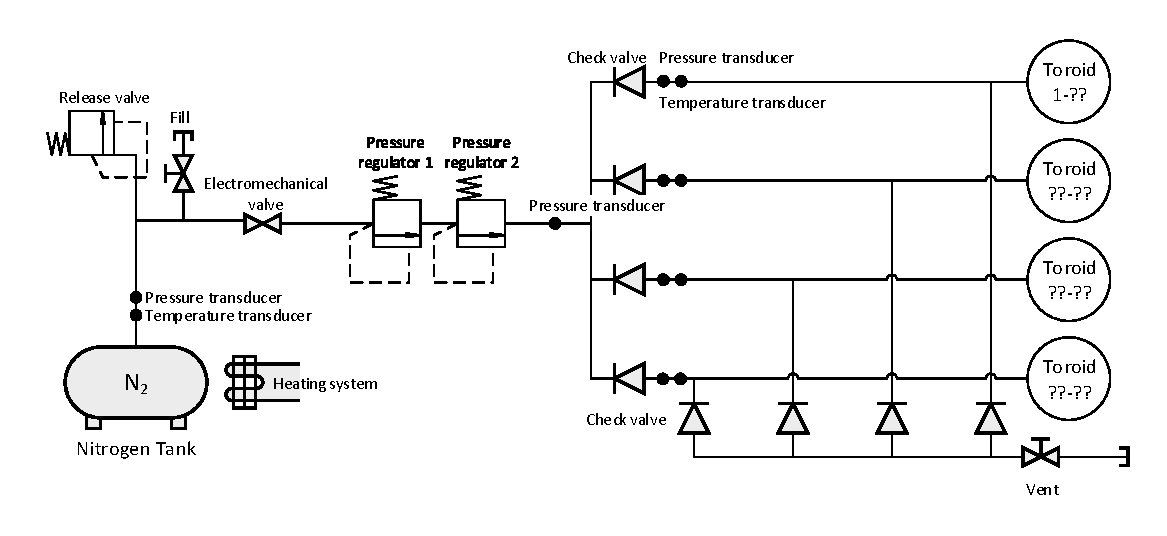
\includegraphics[width=0.95\textwidth]{./Figure/Structure/infsys.pdf}
		\caption[Schematic view of the inflation system]{Schematic view of the inflation system}% (adapted from \cite{Hughes2005})}
		\label{fig:infsys}
\end{figure}


A contingency of $25\%$ of tank mass is included to account for the blow-down system that transfers gas from the tank to the inflatable volumes. For a tank mass of 61 [$kg$], total inflation system mass is 76 [$kg$] to support a gas mass of 90 [$kg$].






